\chapter{$b$-Physics from Lattice NRQCD}

This chapter gives some detail about a number of project attempted using the NRQCD formalism for the $b$ quark. Much of the discussion in this chapter will concern the NRQCD-HISQ representation of the vector and axial $b\to c$ currents, i.e, the current if one of the quarks obeys NRQCD and the other obeys HISQ. We give a number of attempts to improve the normalization of these currents (sections \ref{sec:relativistic}, \ref{sec:Bcetac} and \ref{sec:V0Sf0p}) and an attempt at a calculation of the $B\to Dl\nu$ and $B_s\to D_s l\nu$ form factors (Sec. \ref{sec:BD_BsDs_nrqcd}).

None of the work in this chapter reached a particularly satisfying conclusion. The takehome is that using NRQCD for $b \to c$ currents is riddled with issues. If it can be computationally afforded, an alternative approach like heavy-HISQ is a far simpler and has a stronger grounding.

\section{NRQCD-HISQ currents}

Much of this chapter concerns the nature of the NRQCD-HISQ current, a current with one NRQCD quark and one HISQ quark. To construct such a current, both the HISQ $c$ and NRQCD $b$ must be transformed into 4-component spinors such that they can be contracted with one-another in the current. The staggered $c-$quark $\chi_c$ is simply related to the naive spinor $\psi_c$ by $\psi_c(x)=\gamma_x \chi_c(x)$. The NRQCD $b$, $\Psi_{b} = ( \Psi_+, 0 )$, is a 2-component spinor related to the 4-component spinor $\psi_b$ via an inverse Fouldy-Wouthuysen transform $\psi_b = \exp( - \gamma\cdot \nabla / 2m_b )\Psi_b$.

Due to the Fouldy-Wouthuysen transform, a current $\bar{\psi}_c \Gamma \psi_b$ (where $\Gamma$ is some product of gamma matrices) will be made of an infinite sum of lattice currents in terms of $\Psi_b$, $\bar{\psi}_c \Gamma \psi_b \sim \sum_j (1/m_b^j) \sum_k \bar{\psi}_c \mathcal{O}^{j,k} \Psi_b$. However, this is only half the story - as additionally to the contribution at tree-level from the Fouldy-Wouthuysen expansion, matching the lattice NRQCD theory to continuum QCD gives radiative corrections to this series. Relating continuum QCD currents to lattice NRQCD-HISQ currents causes a 'mixing' of operators as described in Sec. \ref{sec:renormalization}.

So a continuum current $J_{\mu}$ is constructed from a series of the form
\begin{align}
  J_{\mu} = \sum_{j,k} c_j(\alpha_s,am_b) {1\over (2m_b)^j} \bar{\psi}_c \mathcal{O}^{j,k} \Psi_b.
\end{align}
where $j$ sums over powers of inverse $b$-mass and $k$ sums over all operators of dimension $j$. The coefficients $c_j(\alpha_s,am_b)$ are fixed by matching appropriate transition amplitudes in 1-loop continuum QCD and the lattice theory NRQCD/HISQ theory. The vector and axial vector current take the general form \cite{PhysRevD.59.094504};
\begin{align}
	J_{\mu} \,=\, & ( 1 + z^{J_{\mu}}_0 \alpha_s ) J_{\mu,\text{lat}}^{(0)} + ( 1 + z^{J_{\mu}}_1 \alpha_s ) J_{\mu,\text{lat}}^{(1)} \nonumber \\ &+ \alpha_s \sum_{n=2}^4 z^{J_{\mu}}_n J_{\mu,\text{lat}}^{(n)} + \mathcal{O}( \alpha_s^2, (\Lambda_{\text{QCD}}/m_b)^2, (p/m_b)^2 ),
	\label{eq:naive}
        \\
        & J_{\mu,\text{lat}}^{(0)} = \bar{\psi}_c \Gamma_{\mu} \Psi_b,
        \quad\quad J_{\mu,\text{lat}}^{(1)} = -{1\over 2am_b} \bar{\psi}_c \Gamma_{\mu} \gamma\cdot \nabla \Psi_b,
        \nonumber
        \\
        & J_{\mu,\text{lat}}^{(2)} = -{1\over 2am_b} \bar{\psi}_c \gamma\cdot \stackrel{\leftarrow}{\nabla} \Gamma_{\mu} \Psi_b,
        \nonumber
        \quad\quad J_{\mu,\text{lat}}^{(3)} = -{1\over 2am_b} \Gamma_0 \bar{\psi}_c \nabla_{\mu} \Psi_b,
        \nonumber
        \\
        & J_{\mu,\text{lat}}^{(4)} = {1\over 2am_b} \bar{\psi}_c \stackrel{\leftarrow}{\nabla}_{\mu} \Gamma_0 \Psi_b.
        \nonumber
	%% \\ &= ( 1 + z^{J_{\mu}}_0 \alpha_s )( J_{\mu}^{(0)} + J_{\mu}^{(1)} ) + \mathcal{O}( \alpha_s \Lambda_{\text{QCD}} / M, \alpha_s p/M,  \alpha_s^2, (\Lambda_{\text{QCD}}/M)^2, (p/M)^2 ) \\
	%% &= Z^{J_{\mu}}_{J_{\mu}}(1 + z^{J_{\mu}}_0 \alpha_s)( J_{\mu}^{(0)} + J_{\mu}^{(1)} ) \quad,\quad Z^{J_{\mu}}_{J_{\mu}} = 1 + \mathcal{O}(\alpha_s \Lambda_{\text{QCD}} /M, \alpha_s p/M, \alpha_s^2, (\Lambda_{\text{QCD}}/M)^2, (p/M)^2 )
	%% \label{eq:overall}
\end{align}
where $\Gamma_{\mu}$ is the continuum spin structure (e.g. for $A_{\mu}$; $\Gamma_{\mu}=\gamma_5\gamma_{\mu}$) and $p$ is the spacial momentum of the $c$ quark in the current. The last two currents $J^{(3)}_{\mu,\text{lat}}$ and $J^{(4)}_{\mu,\text{lat}}$ do not appear in the temporal current $J_0$, $z_{3,4}^{J_0} = 0$.

The perturbative matching factors $\{z^{J_{\mu}}_n|n=0,1\}$ have been calculated for $V_{\mu}$ and $A_{\mu}$ for the $b\to c$ case in \cite{Monahan:2012dq}. No perturbative result is currently avaliable for $z^{J_{\mu}}_{2,3,4}$. To sidestep this, in studies using these currents an extra truncation in $\alpha_s p/m_b$ is added resulting in
\begin{align}
  J_{\mu} &= ( 1 + z^{J_{\mu}}_0 \alpha_s )( J_{\mu,\text{lat}}^{(0)} + J_{\mu,\text{lat}}^{(1)} ) \\ \nonumber &\quad + \mathcal{O}( \alpha_s \Lambda_{\text{QCD}} / m_b, \alpha_s p/m_b,  \alpha_s^2, (\Lambda_{\text{QCD}}/m_b)^2, (p/m_b)^2 ).
  %% \\
  %% &= Z_{J_{\mu}}(1 + z^{J_{\mu}}_0 \alpha_s)( J_{\mu,\text{lat}}^{(0)} + J_{\mu,\text{lat}}^{(1)} ) \\ &\quad\quad \left( Z_{J_{\mu}} = 1 + \mathcal{O}(\alpha_s \Lambda_{\text{QCD}} /m_b, \alpha_s p/m_b, \alpha_s^2, (\Lambda_{\text{QCD}}/m_b)^2, (p/m_b)^2 ) \right). \nonumber
\end{align}
  One will often then also compute $\langle J_{\mu,\text{lat}}^{(2,3,4)}\rangle$ in the lattice calculation to check that their magnitude is suitably small such that they can be ignored.

\subsection{Relativistic Normalisation of the $b\to c$ temporal axial current}
\label{sec:relativistic}

One would hope that, given the fully relativistic treatment of the light quark, and the relativistically corrected NRQCD heavy quark, that the behaviour of the meson emerging 
from such a calculation (for example in \cite{Dowdall:2011wh},\cite{Colquhoun:2015oha},\cite{Colquhoun:2015mfa}) will be approximately relativistic.

We carried out calculations of correlation functions for a meson resembling the $B_c$ meson. I say 'resembling' since the masses of the valence quarks are often not 
quite the physical $b$ and $c$ quarks, they are shifted in the interest of better statistics, and an extrapolation to physical masses using chiral perturbation theory. Approximate creation operators for this $B_c(x)$ are given by \eqref{eq:meson} 
with $\Gamma = \gamma_5\gamma_0$, and $f(x) \sim \exp(-{x\over\tau})$ for $\tau=a/2\pi,a/4\pi$. 

\begin{table}
\begin{center}
 \begin{tabular}{||c c c c c c c c c||} 
 \hline
 $\beta$ & $a/\text{fm}$ & $am_b$ & $am_c$ & $am_l^{\text{sea}}$ & $am_s^{\text{sea}}$ & $am_c^{\text{sea}}$ & $L_x/a$ & $L_t/a$  \\ [0.5ex] 
 \hline\hline
 6.30 & 0.0884(3) & 1.91 & 0.43 & 0.0074 & 0.037 & 0.440 & 32 & 96 \\ [1ex] 
 \hline
\end{tabular}
\caption{Bare parameters used in this study. $am_b$ and $am_c$ are masses of the valence $b$ and $c$ quarks. $am^{\text{sea}}$ are the masses of quarks in the sea, i.e. contributions from
loop corrections to the gauge field $U$ including these quarks. There are two quarks of mass $l$ (representing $u$ and $d$), and annother two representing $c$ and $s$.}
\end{center}
\end{table}

\subsubsection{Kinetic mass}
\label{sec:kinetic_mass}

The first piece of physics that can be extracted from these parameters is the mass of the meson. If we were using a fully relativistic action, one could simply consider $E^l_0$ (with $\underline{P}=0$) 
to be the mass. However, in our case one would expect NRQCD to cause a shift in energy $E_s$ due to the effective removal of the first term in \eqref{eq:rel_expansion}, so
\begin{align}
 E^l_0(\underline{P}) = E_s + \sqrt{ \underline{P}^2 + M_{B_c}^2 }
 \label{eq:euclidean_energy}
\end{align}
One can then deduce $M_{B_c}$ by taking the difference of energies at different momenta $\delta E^l_0(\underline{p}) \equiv E^l_0(\underline{P}) - E^l_0(0)$, leading to
\begin{align}
 M_{B_c} = { \underline{P}^2 - \delta E_0^{l2} \over 2\delta E^l_0 },
 \label{eq:kinetic_mass}
\end{align}
which should hopefully be invariant of $\underline{P}$. In fig. 2, the mass is deduced from different $\delta E^l_0(\underline{P})$. When deduced in this way $M_{B_c}$ is 
referred to as the \textit{kinetic mass}.
\begin{center}
\begin{figure}
\begin{tikzpicture}
\begin{axis}[width=10cm,height=8cm,
		xlabel=$(a\underline{P})^2$, ylabel=$aM_{B_c}$]

\addplot+[only marks, color=blue, 
		error bars/.cd,x dir=both, x explicit,  y dir=both, y explicit]
		coordinates {
			(0.02891, 2.61 ) +- (0, 0.11)
			(0.26023, 2.838 )   +- (0, 0.027 )
			(0.72425, 2.823 )   +- (0, 0.014)
			(1.04076, 2.840 ) +- (0, 0.015)
			};
\end{axis}
\end{tikzpicture}
\label{fig:k_mass}
\caption{Meson mass deduced from \eqref{eq:kinetic_mass}}
\end{figure}
\end{center}
We disregard the first point (smallest momentum) assuming the smallness of $\delta E^l_0$ to cause large fractional error in it and therefore in $M_{B_c}$. Averaing over the other three points gives
$aM_{B_c} = 2.834(11)$.

\subsubsection{Decay amplitudes}

If the annihilation operator $B_c$ is made to be local ($f(\underline{x}_n)=\delta_{n0}$), it becomes a temporal axial current operator $A_0$ (the second term in $J^{bc}_0$ 
in the language of sec. \ref{sec:cp}). Then, by setting the creation operator $B_c^{\dagger}$ to be smeared and with a finite 
momentum $\underline{P}$, we can assert that $a_0$ is proportional to the decay amplitude;
\begin{align}
	a_0 = a_0(\underline{P}) = {\langle 0 | A_0 | B_c(\underline{P}) \rangle \over \sqrt{2E^r_{B_c}(\underline{P})} } 
	= {f_{B_c} E^r_{B_c}(\underline{P}) \over \sqrt{2E^r_{B_c}(\underline{P})}} = f_{B_c} \sqrt{2E^r_{B_c}(\underline{P})}.
\end{align}
The second equality is from the fact that since $A_{\mu}$ is a conserved current, and has one Lorentz index, it must be proportional to the meson's 4-momentum, 
$\langle A_{\mu} \rangle \propto P_{\mu}$. $f_{B_c}$ is the $B_c$ decay constant.

We hope that, if the lattice calculation is well designed and the 
bare parameters in the actions are well chosen, that this equality will hold to a good approximation, supplying us with a new piece of evidence that results 
from such calculations can be considered relevant to real physics.

Our probe of the relativistic normalisation is the ratio:
\begin{align}
	{a_0(\underline{p})\over a_0(0)} & = {\langle 0 | A_0 | B_c(\underline{P}) \rangle \over \langle 0 | A_0 | B_c(0) \rangle} = 
	\sqrt{E^r_{B_c}(\underline{P})\over M_{B_c}} = 1 + {\underline{P}^2\over 4M_{B_c}^2} + \mathcal{O}\left({\underline{P}^4\over M_{B_c}^4}\right),
	\label{eq:relativistic_meson}
\end{align}
Where $a_0(\underline{P})$ comes from fits of $C_{B_c}(t,\underline{P})$.
We fitted correlation functions at different spacial momenta, deduced many $a_0(\underline{P})$ values, took the ratio with $a_0(0)$ and compared to 
\eqref{eq:relativistic_meson} (see the $a^{(0)}_1(\underline{P})/a^{(0)}_1(0)$ line in fig. \ref{fig:relativistic}).

\begin{figure}
\begin{center}
	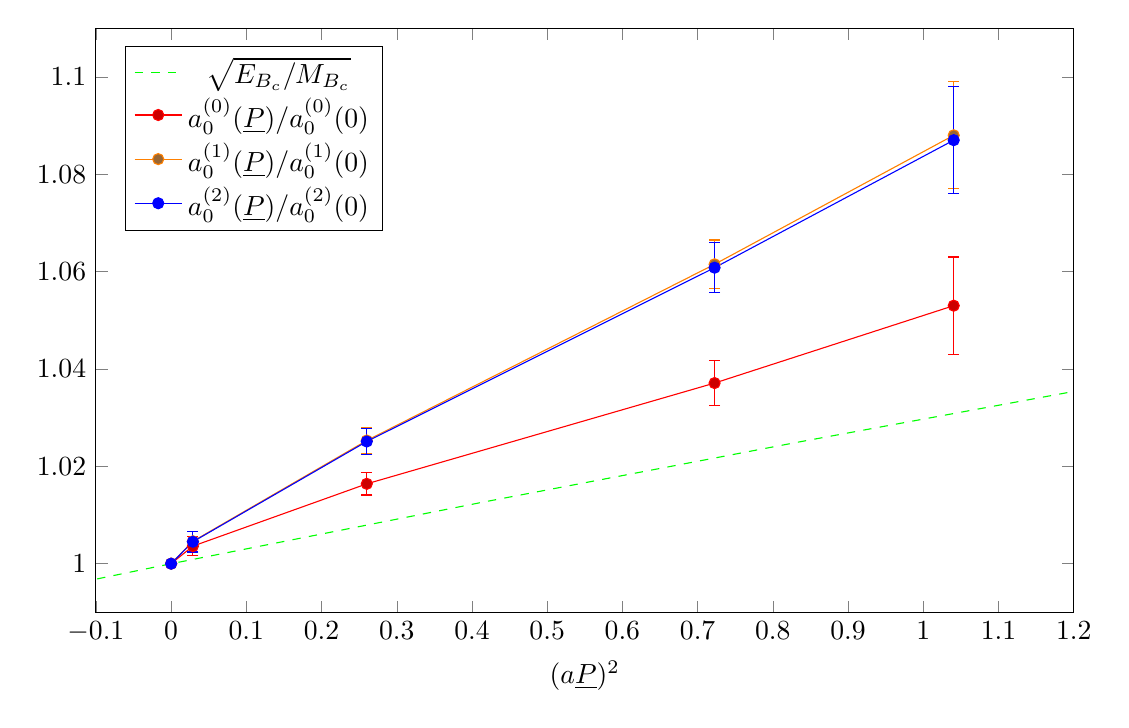
\begin{tikzpicture}
		\begin{axis} [width=14cm,height=9cm,
			xmin=-0.1,xmax=1.2,ymin=0.99,ymax=1.11,
			xlabel = $(a\underline{P})^2$, 
			legend pos=north west]
			
			\addplot[color=green, dashed]{ sqrt( sqrt( x + 2.834*2.834 )/2.834) };
			\addlegendentry{$\sqrt{E_{B_c}/M_{B_c}}$}
			
			\addplot+[color=red, mark=*, 
					error bars/.cd,x dir=both, x explicit,  y dir=both, y explicit] 
				coordinates {
					(0, 1)   +- (0, 0)
					(0.02890, 1.0036)   +- (0.0, 0.0019)
					(0.26010, 1.0164)   +- (0.0, 0.0023)
					(0.7225, 1.0371)   +- (0.0, 0.0046)
					(1.0404, 1.053)   +- (0.0, 0.01)
			};
			\addlegendentry{$a_0^{(0)}(\underline{P})/a_0^{(0)}(0)$}
			
			\addplot+[color=orange, mark=*, 
					error bars/.cd,x dir=both, x explicit,  y dir=both, y explicit] 
				coordinates {
					(0, 1)   +- (0, 0)
					(0.02890, 1.0046)   +- (0.0, 0.0021)
					(0.26010, 1.0253)   +- (0.0, 0.0026)
					(0.7225, 1.0615)   +- (0.0, 0.0050)
					(1.0404, 1.088)   +- (0.0, 0.011)
			};
			\addlegendentry{$a_0^{(1)}(\underline{P})/a_0^{(1)}(0)$}
			
			\addplot+[color=blue, mark=*, 
					error bars/.cd,x dir=both, x explicit,  y dir=both, y explicit] 
				coordinates {
					(0, 1)   +- (0, 0)
					(0.02890, 1.0045)   +- (0.0, 0.0021)
					(0.26010, 1.0251)   +- (0.0, 0.0026)
					(0.7225, 1.0608)   +- (0.0, 0.0051)
					(1.0404, 1.087)   +- (0.0, 0.011)
			};
			\addlegendentry{$a_0^{(2)}(\underline{P})/a_0^{(2)}(0)$}
			
		\end{axis}
	\end{tikzpicture}
\end{center}
\caption{Relativistic Normalisation of 1-loop corrected Axial Current. $a_0^{(n)}$ are defined in \eqref{eq:a_0corrections}. }
  \label{fig:relativistic}
\end{figure}

\subsubsection{Operator Matching}

In \cite{Morningstar:1997ep}, it is shown that this operator for the axial current by itself on the lattice is not totally sufficient to represent a continuum axial current. 
In this paper, the axial vector current with 1-loop corrections in continuum QCD (illustrated in figure 1, 2 and 3 in \cite{Morningstar:1997ep}) was computed using the on-shell mass and wave function renormalisation scheme in Feynman gauge. The light quark on-shell mass was approximated to zero, and the result was expanded in powers of the inverse heavy quark on-shell mass $1/M$.
\begin{align}
	\nonumber
	\langle q(p') | A_0 | h(p) \rangle_{\text{QCD}} = & \eta_1 [ \bar{u}_q(p') \gamma_5\gamma_0 u_h(p) ] + \eta_2 \left[ {p_0\over M} \bar{u}_h(p') \gamma_5 u_h(p) \right] \\
	\nonumber
	+ & \eta_3\left[ {p\cdot p'\over M^2} \bar{u}_q (p') \gamma_5\gamma_0 u_h(p)\right]
	 + \eta_4\left[{p_0'\over M} \bar{u}_q(p') \gamma_5 u_h(p)\right] \\
	 + & \mathcal{O}\left({1\over M^3}\right) \\ \nonumber \\
	 \nonumber
	 \eta_1 =  1 + &{\alpha_s\over 3\pi}\left[ 3\ln {M\over \lambda} - {11\over4} \right] \quad,\quad \eta_2 = {\alpha_s\over 3\pi} 2 \\
	 \nonumber
	 \eta_3 = {\alpha_s\over 3\pi} &\left[ 6\ln {M\over\lambda} - {8\pi\over 3}{M\over\lambda} + {1\over 2} \right] \quad,\quad \eta_4 = {\alpha_s\over 3\pi} \left[ -2 \ln {M\over \lambda} + {1\over 2} \right]
	 \label{eq:continuum_axial}
\end{align}
$\lambda$ is the artificial Gluon mass (should cancel in obeservables), $|q(p')\rangle$ and $|h(p)\rangle$ are asymptotic light and heavy quark states respectively, and $u_{q,h}$ are the corresponding fermion wavefunctions. 

The dimensional requirements that $1/M$ must always come with a power of momenta turns this $1/M$ expansion into an expansion in velocity $v$, so is an NRQCD expansion. There are two expansions at play: $v$ and $\alpha_s$, one should avoid mixing them up.

In our lattice simulation the heavy quark obeys NRQCD so only has 2 components (there is no antiparticle without a relativistic dispersion relation). The particle and antiparticle fields in $h(x)$ can be decoupled using the Fouldy-Wouthuysen (FW) transformation \cite{Foldy:1949wa}, which is a canonical transformation, i.e. a change of variables of $h(x)$'s spinor degrees of freedom. Using the FW transformation, one can relate the $u_h$ to the wavefunction of a 2 component quark $U_h(p)$:
\begin{align}
	u_h(p) = \exp\left(-{\underline{\gamma}\cdot\underline{p}\over 2M}\right) \binom{U_h(p)}{0}
%	\label{eq:FW}
\end{align}
Using this to replace $u_h$ with $U_h$ in \eqref{eq:continuum_axial}, and inspecting the form of the leading order contributions, one can identify operators in the lattice theory that should be used to reproduce the continuum axial current $A_0$ \cite{Dowdall:2013tga}:
\begin{align}
	&A_0 = (1+z_0 \alpha_s ) \left[ A_{0,\text{lat}}^{(0)} + (1 + z_1\alpha_s) A_{0,\text{lat}}^{(1)} + z_2\alpha_s A_{0,\text{lat}}^{(2)} \right]
	\label{eq:current_corrections}
\\	&A_{0,\text{lat}}^{(0)} = \bar{c} \gamma_5 \gamma_0 b
	\nonumber
\\	&A_{0,\text{lat}}^{(1)} = -{1\over2m_b} \bar{c} \gamma_5 \gamma_0 \underline{\gamma}\cdot\underline{\nabla} b
	\nonumber
\\	&A_{0,\text{lat}}^{(2)} = -{1\over2m_b} \bar{c} \underline{\gamma}\cdot\underline{\overleftarrow{\nabla}} \gamma_5 \gamma_0  b.
	\nonumber
\end{align}
$c$ and $b$ are the quark creation operators. The mass $M$ has been replaced with the bare $b$ mass $m_b$, since the on-shell mass only exists in perturbation theory so has no meaning in terms of the lattice. 
The coefficients $\{z_i\}$ can be obtained from matching terms between continuum and lattice perturbation theory.

The values $\{z\}$ are not yet known for the $bc$ current, but to give an idea of order or magnitude, in fig. \ref{fig:relativistic} uses values from the temporal axial current between light and $b$ quarks. Taken from \cite{Dowdall:2013tga}, these are $z_0=-0.007(2)$, $z_1=-0.031(4)$, $z_2=-0.325(4)$. $\alpha_s = 0.267$ is taken from set 7 of \cite{Colquhoun:2015oha}, obtained from running down of $\alpha_s^{\overline{MS}}(M_Z)$ down to scales of the simulation dictated by $a$.

$A_{0,\text{lat}}^{(0)}$ is the naive current operator used before (i.e with local smearing $\tilde{B}_c = A_{0,\text{lat}}^{(0)}$ in \eqref{eq:correlator}). 
To calculate the corrections, 
this was replaced with $A_{0,\text{lat}}^{(1,2)}$, and the calculation and fitting was repeated to extract $a_0$, this time coenciding with 
$\langle 0 | A_{0,\text{lat}}^{(1,2)} | B_c(\underline{P}) \rangle$. From these values one can build up a better estimation to the continuum current 
$\langle 0 | A_0 | B_c(\underline{P}) \rangle$. In fig. \ref{fig:relativistic} we gradually add corrections to see the effect each has, defining
\begin{align}
  \nonumber
  \label{eq:a_0corrections}
  &a_0^{(0)} = \langle 0 | (1+z_0 \alpha_s ) A_{0,\text{lat}}^{(0)} | B_c(\underline{P}) \rangle \\
  &a_0^{(1)} = \langle 0 | (1+z_0 \alpha_s ) \left[ A_{0,\text{lat}}^{(0)} + (1 + z_1\alpha_s) A_{0,\text{lat}}^{(1)} \right] | B_c(\underline{P}) \rangle \\
  \nonumber
  &a_0^{(2)} = \langle 0 | (1+z_0 \alpha_s ) \left[ A_{0,\text{lat}}^{(0)} + (1 + z_1\alpha_s) A_{0,\text{lat}}^{(1)} + z_2\alpha_s A_{0,\text{lat}}^{(2)} \right] | B_c(\underline{P}) \rangle \\
  \nonumber
\end{align}

%% \begin{table}
%% \begin{center}
%%  \begin{tabular}{||c c c c c c c c c||} 
%%  \hline
%%  set & $(a\underline{P})^2$ & $a\delta E_0(\underline{P})$  & $aM_{B_c}$ & $a_0^{(0)}(\underline{P})/a_0^{(0)}(0)$ & $a_0^{(1)}(\underline{P})/a_0^{(1)}(0)$ 
%%  & $a_0^{(2)}(\underline{P})/a_0^{(2)}(0)$ \\ [0.5ex] 
%%  \hline\hline
%%  1 & 0.02891 & 0.00537(23) & 2.61(11) & 1.0036(19) & 1.0046(21) & 1.0045(21) \\ \hline
%%  2 & 0.26023 & 0.04580(24) & 2.838(27) & 1.0164(23) & 1.0253(26) & 1.0251(26) \\ \hline
%%  3 & 0.72287 & 0.12456(46) & 2.823(14) & 1.0371(46) & 1.0615(50) & 1.0608(51) \\ \hline
%%  4 & 1.04093 & 0.17772(86) & 2.840(15) & 1.053(10) & 1.088(11) & 1.086(11) \\ [1ex] 
%%  \hline
%% \end{tabular}
%% \end{center}
%% \caption{Results from fits with varying momenta. The third column gives the kinetic mass deduced from $\delta E(\underline{P})$ for each $\underline{P}$. using \eqref{eq:kinetic_mass}\label{tab:from_fit}}
%% \end{table}
As one adds these current corrections, one would expect the resulting ratio's $\underline{P}$-dependance to move closer to \eqref{eq:relativistic_meson}. This can also be considered to be a 
test of the coefficients $\{ z_i \}$, since we could in principle tune them in this calculation until the results coincide with the expected relativistic expression.
\\ \\
As can be seen from fig. \ref{fig:relativistic}, The effect of the correction terms is not what was hoped, it seems to move the ratio away from the physical relation. 
An unnatrually large modification to the $\{z_i\}$ values would be required to coincide this ratio with the physical one. It is clear that the effect of these correction terms are not well understood.
\\ \\
It is possible that the masses of the light and heavy quark in these calculations were too close to each other. In the deduction of \eqref{eq:current_corrections}, $m_c$ is 
approximated to zero and $m_b$ is assumed large enough so that a truncation to order $1/m_b^2$ is a good approximation. Hence, we have started investigating the effect on this 
ratio due to a reduction in the mass of the charm quark.

\subsubsection{$A_0^{(3)}$ contribution}

These current corrections are only to $\mathcal{O}(\underline{p}_b/m_b)$, but $\sqrt{E^r_{B_c}/M_{B_c}}$ has it's leading behaviour in $\mathcal{O}(\underline{P}^2/M_{B_c}^2)$. This implies one needs to carry on the expansion of current corrections further, to $\mathcal{O}(1/m_b^2)$. The dominant term at this order arises at tree level from the first term in \eqref{eq:continuum_axial}, and the second term in a $1/M$ expansion of \eqref{eq:FW}. The corresponding lattice operator is
\begin{align}
	A^{(3)}_{0,\text{lat}} = {1\over 8m_b^2} \bar{c} \gamma_5\gamma_0 \underline{\nabla}^2 b. 
\end{align}
This was computed in a lattice calculation and combined with the lower orders to produce $a^{(3)}_0 = a_0^{(2)} + A^{(3)}_{0,\text{lat}}$. In this case we set $\alpha_s = 0$ to just focus on tree level. The results are shown on fig. \ref{fig:A3}.
\begin{figure}
\begin{center}
    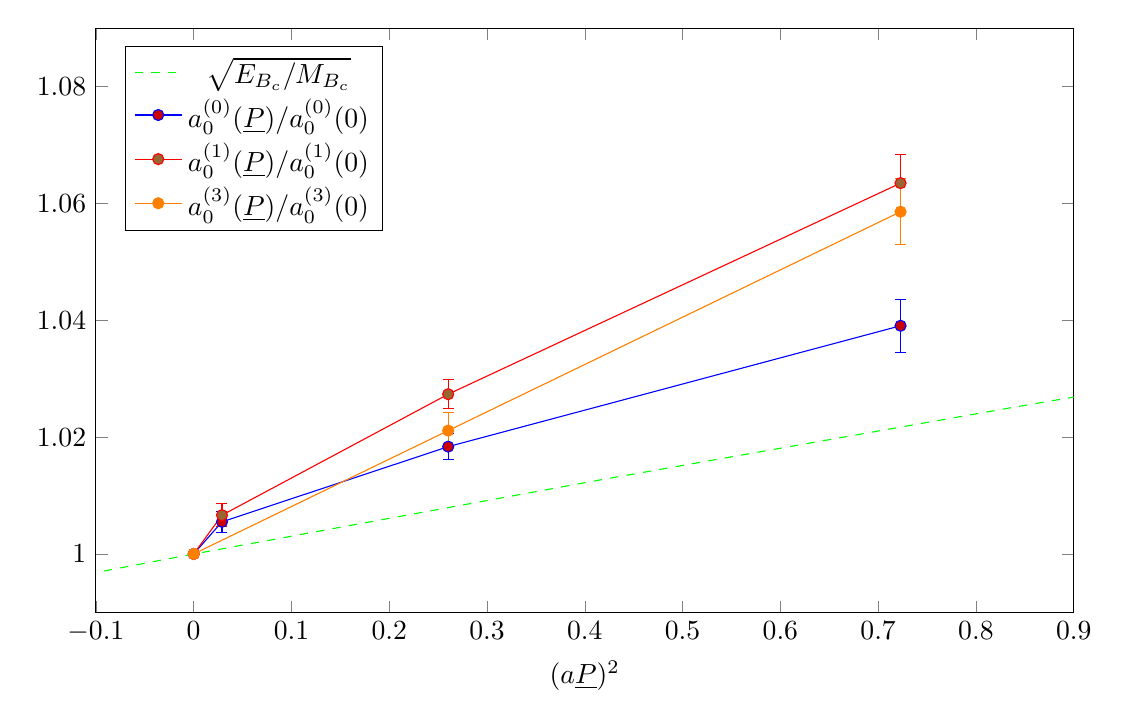
\begin{tikzpicture}
        \begin{axis} [width=14cm,height=9cm,
            xmin=-0.1,xmax=0.9,ymin=0.99,ymax=1.09,
            xlabel = $(a\underline{P})^2$,
            legend pos=north west]

            \addplot[color=green, dashed]{ sqrt( sqrt( x + 2.834*2.834 )/2.834) };
            \addlegendentry{$\sqrt{E_{B_c}/M_{B_c}}$}

            \addplot+[color=blue, mark=*,
                    error bars/.cd,x dir=both, x explicit,  y dir=both, y explicit]
                coordinates {
                		(  0.0 ,  1.0  ) +- ( 0.0,  1.33226762955e-19  )
		  	(  0.0289148446127 ,  1.00549267643  ) +- ( 0.0,  0.00176452228481  )
			(  0.260233601514 ,  1.01836440302  ) +- ( 0.0,  0.00222088535291  )
			(  0.722871115317 ,  1.0390590324  ) +- ( 0.0,  0.00452197676768  )
            };
            \addlegendentry{$a_0^{(0)}(\underline{P})/a_0^{(0)}(0)$}

            \addplot+[color=red, mark=*,
                    error bars/.cd,x dir=both, x explicit,  y dir=both, y explicit]
                coordinates {
                		(  0.0 ,  1.0  ) +- ( 0.0,  0.0  )
          	        (  0.0289148446127 ,  1.00663334793  ) +- ( 0.0,  0.00194538583335  )
			(  0.260233601514 ,  1.02734203998  ) +- ( 0.0,  0.00244820981549  )
			(  0.722871115317 ,  1.06347584999  ) +- ( 0.0,  0.00497690081001  )
            };
            \addlegendentry{$a_0^{(1)}(\underline{P})/a_0^{(1)}(0)$}
            
            \addplot+[color=orange, mark=*,
                    error bars/.cd,x dir=both, x explicit,  y dir=both, y explicit]
                coordinates {
                		(  0.0 ,  1.0  ) +- ( 0.0,  0.0  )
			(  0.260233601514 ,  1.0211157939  ) +- ( 0.0,  0.00302333986783  )
			(  0.722871115317 ,  1.05858288737  ) +- ( 0.0,  0.00568371480017  )
            };
            \addlegendentry{$a_0^{(3)}(\underline{P})/a_0^{(3)}(0)$}

        \end{axis}
    \end{tikzpicture}
\end{center}
\caption{Relativistic Normalisation of 1-loop corrected Axial Current. $a_0^{(n)}$ are defined in \eqref{eq:a_0corrections}. (tree level) }
\label{fig:A3}
\end{figure}
As a sanity check for the $A^{(3)}$ calculation, fig. \ref{fig:A3A2} shows the ratio $A^{(3)}_{0,\text{lat}}(\underline{P})/A^{(2,1)}_{0,\text{lat}}(\underline{P})$. Since $A^{(3)} = \mathcal{O}(\underline{p}^2)$ and $A^{(1)} = \mathcal{O}(\underline{p})$, we expect such a ratio to be proportional to $|\underline{p}|$ (see fig. \ref{fig:A3A1}). {\color{red}{The $A^{(3)}/A^{(2)}$ line isn't straight...}}

%==========
\begin{figure}
\begin{center}
    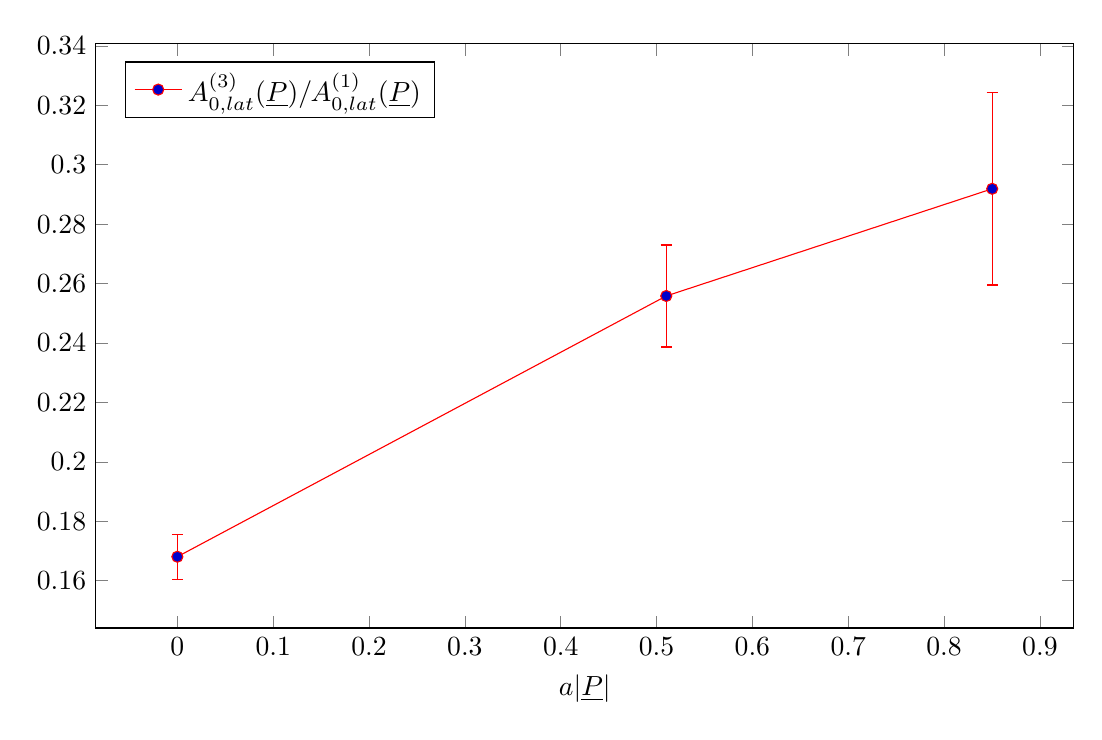
\begin{tikzpicture}
        \begin{axis} [width=14cm,height=9cm,
            xlabel = $a|\underline{P}|$,
            legend pos=north west]

            \addplot+[color=red, mark=*,
                    error bars/.cd,x dir=both, x explicit,  y dir=both, y explicit]
                coordinates {
               		(  0.0 ,  0.168061897514  ) +- ( 0.0,  0.00761364082979  )
			(  0.510130965061 ,  0.255812358549  ) +- ( 0.0,  0.0171547894616  )
			(  0.850218275102 ,  0.291882276843  ) +- ( 0.0,  0.0323767757253  )
                    
            };
\addlegendentry{$A^{(3)}_{0,\text{lat}}(\underline{P})/A^{(1)}_{0,\text{lat}}(\underline{P})$}

        \end{axis}
    \end{tikzpicture}
\end{center}
\label{fig:A3A1}
\caption{Ratio of third current correction to first.}
\end{figure} 

\section{$B_{(s)}\to D_{(s)}l\nu$ form factors}
\label{sec:BD_BsDs_nrqcd}

\subsection{Lattice Setup}

\begin{table}
\begin{center}
 \begin{tabular}{||c c c c c c c c||}
 \hline
 Set & $a/\text{fm}$ & $am_l$ & $am_s$ & $am_c$ & $L_x/a$ & $L_t/a$ & $N_{\text{cfg}}$ \\ [0.5ex] 
 \hline\hline
 1 & 0.1474(15) & 0.013 & 0.065 & 0.838 & 16 & 48 & 1020 \\ [1ex]
 2 & 0.1219(9) & 0.0102 & 0.0509 & 0.635 & 24 & 64 & 1053 \\ [1ex]
 3 & 0.0884(6) & 0.0074 & 0.037 & 0.440 & 32 & 96 & 1008 \\ [1ex]
 \hline
\end{tabular}
\caption{Parameters for gauge ensembles \cite{Bazavov:2012xda}.
$a$ is the lattice spacing, deduced from a study of the
$\Upsilon$-$\Upsilon'$ splitting \cite{Dowdall:2011wh}. $L_x$ is the spacial extent and $L_t$ the
temporal extent of the lattice. The masses of up, down, stange and
charm quarks included in the sea are given as the dimensionless quantity $am$.
Up and down quarks are taken to have the same mass, $am_l$. $N_{\text{cfg}}$ is the number of configurations in the ensemble. We calculate propagators from 16 time sources on each ensemble to increase statistics. \label{tab:nrqcdensembles}}
\end{center}
\end{table}

\begin{table}
\begin{center}
 \begin{tabular}{||c c c c c c c c c c||}
 \hline
 Set & $am_s$ & $am_c$ & $am_b$ & $u_0$ & $\epsilon_{\text{Naik}}$ & $c_{1,6}$ & $c_5$ & $c_4$ & $\{T\}$ \\ [0.5ex] 
 \hline\hline
 1 & 0.0705 & 0.826 & 3.297 & 0.8195 & -0.3449 & 1.36 & 1.21 & 1.22 & 8, 11, 14 \\ [1ex]
 2 & 0.0541 & 0.645 & 2.66 & 0.8340 & -0.2348 & 1.31 & 1.16 & 1.20 & 9, 12, 15 \\ [1ex]
 3 & 0.0376 & 0.450 & 1.91 & 0.8525 & -0.1256 & 1.21 & 1.12 & 1.16 & 14, 19, 24 \\ [1ex]
 \hline
\end{tabular}
\caption{Parameters used in our calculation. $am_s$ and $am_c$ are the bare masses of the strange, charm valence quarks, tuned in \cite{PhysRevD.91.054508}, $am_b$ is the bare mass of the valence bottom quark, tuned in \cite{Dowdall:2011wh}
$u_0$ is the 'tadpole improvement parameter' as used in \cite{Dowdall:2011wh}.
$\epsilon_{\text{Naik}}$ is the Naik parameter in the HISQ action \cite{Follana:2006rc}.
$\{c_i\}$ are the coefficients for the kinetic and chromomagnetic terms in the NRQCD action \cite{Hammant:2013sca}. $\{T\}$
is the set of temporal seperations between source ($B_s$ creation operator) and sink ($D_s$ anihilation operator). \label{table:quarkmasses}
}
\end{center}
\end{table}

We follow a largely similar approach to the recent $B\to Dl\nu$ and $B_s\to D_sl\nu$ calculations in \cite{Na:2015kha} and \cite{Monahan:2017uby}.
\\ \\
Table \ref{tab:nrqcdensembles} gives details of the ensembles used in this study. These are taken from the MILC HISQ ensembles \cite{Bazavov:2012xda}. They are generated by MCMC with the distribution given in \eqref{eq:MCweight}, where $M$ is the Dirac operator for the HISQ action. They take into accound up, down, strange and charm quarks, assuming the contribution from higher mass quarks in the sea to be negligable.
\\ \\
Following the procedure discussed in section \ref{sec:correlators}, first we must compute 2-point correlators for the $B_s$ and $D_s$. In both cases we use \textit{smeared} creation operators:
\begin{align}
	\Phi^{\alpha}(\underline{k},t) = \sum_{\underline{x},\underline{x'}} e^{-i\underline{k}\cdot\underline{x}} \text{ } \bar{\psi}_1(\underline{x'},t)\phi^{\alpha}(\underline{x}'-\underline{x}) \gamma_5 \psi_2(\underline{x})
\end{align}
where $\bar{\psi}_1$,$\psi_2$ are $\bar{b}$,$s$ for the $B_s$ and $\bar{c}$,$s$ for the $D_s$. The smearing functions $\phi^{\alpha}$ approximate the wavefunction of one quark in a potential set up by the other, giving a psuedo-realistic representation of the meson. This makes the operator $\Phi^{\alpha}$ couple stronger to the ground state of the meson, maximizing the $a_0 \propto \langle0 |\Phi^{\alpha}|\lambda_0\rangle$ parameter in the fit \eqref{eq:multiexponential} relative to the excited states $a_{n>0}$. This increases the dominance of the first term in \eqref{eq:multiexponential} resulting in better convergence of the $n$ sum, therefore a better fit and better statistics of the results.
\\ \\
For the $B_s$, we use a combination of $\phi^0(\underline{z})=\delta(\underline{z})$ ("local"), and $\phi^{1,2}(\underline{z}) \propto \text{exp}(-|\underline{z}|/r_0)$ ("smeared"), with $r_0 \simeq 2.5$fm$, 5$fm. For the $D_s$ we use one local and one smeared with $r_0\simeq2.5$fm. Correlation functions between each smearing combination is calculated, i.e. for the $D_s$, we compute 4 correlators $\langle \Phi^{0\dagger}_D\Phi_D^0 \rangle$, $\langle \Phi^{1\dagger}_D\Phi_D^0 \rangle$, $\langle \Phi^{0\dagger}_D\Phi_D^1 \rangle$, $\langle \Phi^{1\dagger}_D\Phi_D^1 \rangle$, and 9 for the $B_s$.
\\ \\
A good way to see the benefit of the smearing is by plotting the effective mass $m_{\text{eff}}(t) = \text{log}({C(t)/C(t+1)})$ against $t$ as in fig. \ref{fig:effmass}. The flatness of this as a function in $t$ shows how well it is approximated by the fit function with only the ground state (i.e. not contaminated by excited states), therefore how easily the fit will determine the ground-state energy. As can be seen, The smeared effective mass "flattens out" quicker than the local, as the smeared couples mostly to the ground state.
\\ \\
\begin{figure}
  \begin{center}
    \includegraphics[width=0.65\textwidth]{images/NRQCD/EffMass_localVsSmear_Ds_coarse.png}
  \end{center}
  \caption{Effective mass of $D_s$ correlation functions, one with local $D_s$ operators $\langle\Phi^0\Phi^0\rangle$ and one with smeared $\langle\Phi^1\Phi^1\rangle$.}
  \label{fig:effmass}
\end{figure}

The 3pt correlation function calculated is $\langle \Phi^{\alpha\dagger}_{D_s} V_{\mu} \Phi^{\beta}_{B_s} \rangle$, including all smearings of the $B_s$ and $D_s$ used in the 2-point functions. We must be careful choosing the appropriate operator for $V_{\mu}$. Recall that NRQCD quarks contain an inverse Fouldy-Wouthuysen (FW) transformation \eqref{eq:FoldyWoldy}. This must be encorparated into the $V_{\mu}$ operator, since it couples to the $b$ which obeys the NRQCD action in our simulation. Hence the $V_{\mu}$ operator must be of the form
\begin{align}
	V_{\mu} = \bar{c}\gamma_{\mu}\left( 1 - {1\over 2m_b} \underline{\gamma}\cdot\underline{\nabla} + \mathcal{O}\left({1\over m_b^2}\right) \right) b 
\end{align}
where we can afford to expand the exponential in the FW transformation since $1/m_b$ is small. However, this is only a tree level result. According to the discussion in sec. \ref{sec:renormalization}, these terms require renormalization constants, and also new terms in the above expansion may appear. Therefore the full expression for the vector current that we use is (accurate to $\mathcal{O}(\alpha_s,1/m_b)$):
\begin{align}
	\nonumber
	V_{\mu} &= (1+z_0 \alpha_s)\left[ V_{\mu}^{(0)} + (1 + z_1 \alpha_s) V_{\mu}^{(1)} + z_2 \alpha_s V_{\mu}^{(2)} \right] \\
	\nonumber
	& V_{\mu}^{(0)} = \bar{c}\gamma_{\mu} b \\
	\nonumber
	& V_{\mu}^{(1)} = -{1\over 2m_b} \bar{c} \gamma_{\mu}\underline{\gamma}\cdot\underline{\nabla} b \\
	\nonumber
	& V_{\mu}^{(2)} = -{1\over 2m_b} \bar{c} \gamma_{\mu}\underline{\gamma}\cdot\underline{\overleftarrow{\nabla}} b \\
	\label{eq:currentcorrections}
\end{align}
The coefficients $\{z_i\}$ are set by a matching procedure between the HISQ/NRQCD currents and continuum QCD in \cite{Monahan:2012dq}. We calculate correlation functions $\langle \Phi_{D_s} V^{(i)}_{\mu} \Phi_{B_s}\rangle$ for each current and combine them after the fitting procedure.

\subsection{Deduction of Form Factors}

We wish to use these currents to deduce the $B_s\to D_s l\nu$ form factors discussed in section \ref{sec:formfactors} over the full $q^2$ range. To this end, the above procedure to compute $\langle D_s | V^{(i)}_{\mu} | B_s \rangle$ is repeated while giving the $D_s$ meson a range of different spacial momenta. We chose spacial momentum $\underline{p} = |\underline{p}|(1,1,1)$, in this each direction is equivilant, and it allows us to average $V_{\mu}$ over the 3 spacial directions, reducing work in the fit and increasing the statistics of the averaged current $V_k \equiv \sum_{i=1}^3 V_i / 3$.
\\ \\
As discussed in appendix \ref{sec:signalnoise}, the most accurate results will come from $|\underline{p}| = 0$, then the correlators become noise-dominated as one increases $|\underline{p}|$ towards $|\underline{p}|_{\text{max}}$. Hence, the approach is to start at the $|\underline{p}|=0$ end and move up in momentum, monitoring statistical errors as you go. So far we have performed runs for $|a\underline{p}| = 0,0.30,0.45$ on the fine ensemble, and $|a\underline{p}|=0,0.25,0.50$ on the coarse ensemble. Statistical errors have not yet become uncontrollable at these momenta, but from experience of previous calculations, they are expected to become problematic at $|a\underline{p}| \sim 0.7$. 
\\ \\
With values for $\langle D_s | V_{\mu} | B_s \rangle$ at varying $\underline{p}$ therefore varying $q^2$, we can perform a fit of this data in order to extract $f_{0,+}(q^2)$ via \eqref{eq:formfactors}. To do the fit, we need some anzats for the functional form of $f_{0,+}(q^2)$. We use the BCL parameterization \cite{PhysRevD.79.013008}. This involves first reparameterizing $q^2$ to 
\begin{align}
	z(q^2) = {\sqrt{t_+ - q^2} - \sqrt{t_+ - t_0} \over \sqrt{t_+ - q^2} + \sqrt{t_+ - t_0} }
\end{align}
where we take $t_0 = t_+( 1 - \sqrt{1 - t_-/t_+})$, and $t_{\pm} = (M_{B_s} \pm M_{D_s})^2$, as in \cite{Hill:2006ub}. $z(q^2)$ has a very small magnitude throughout the entire $q^2$ range, in our case $|z|_{\text{max}} \sim 0.032$. We can then accurately model $f_{+,0}$ as a series expansion in $z$:
\begin{align}
	f_{0,+}(q^2) = {1\over P_{0,+}(q^2)} \sum_n a^{0,+}_n z(q^2)^n
	\label{eq:zexpansion}
\end{align}
we truncate this at $z^2$, adding further terms have no effect on the fit. The so-called Blaschke factors $P(q^2)$
are defined by
\begin{align}
	P_{0,+}(q^2) = \left( 1 - {q^2\over M_{0,+}^2}\right)
\end{align}
These are required due to subthreshold poles in the crossed channel of $\langle D_s | V^{(i)}_{\mu} | B_s \rangle$, which in our case is a $W$ decay into a $B_c$ meson. The pole is located where the $W$ has the correct momentum $q^2$ to create the $B_c$, hence at $q^2=M_{B_c}$. This is not within the $q^2$ range, but can create curvature in $f_{0,+}$ that can confound the expansion in $z$. $P_{0,+}$ effectively removes this pole from the $z$ expansion.

\subsection{Continuum \& Chiral Extrapolation}

The form factors $f_{0,+}(q^2)$ we deduce from the above will contain systematic errors due to 1) discretization, and 2) unphysical quark masses and mistunings. 
\\ \\
2) requires a little explaination. In lattice simulations it is computationally expedient (and sometimes neccesary) to take the up/down quark masses $m_l$ to be much larger than their physical values. This is because the condition number of the Dirac operator $M_l$ is proportional to $am_l$, a small condition number makes it difficult or impossible to numerically invert $M_l$ to obtain the propagator $M^{-1}_l$ as part of the process in section \ref{sec:correlators}. Fortunately, since the $B_s\to D_s l\nu$ decay involves no up/down valence quarks, we mostly need not worry about this problem. There is also the issue of mistuning: the quark masses we use are tuned by a calculation of some process, see caption in table \ref{table:quarkmasses}. The uncertainty in these determinations must be accounted for somehow.
\\ \\
The above issues are in general dealt with by computing the above form factors at a number of lattice spacings and quark masses, and results extrapolated to $a\to 0$ and $m\to m_{\text{physical}}$. The $a\to 0$ extrapolation is performed by involving data from all ensembles in the fit to $f_{0,+}$, and modifying \eqref{eq:zexpansion}:
\begin{align}
	a^{0,+}_n \to a^{0,+}_n \times ( 1 + b^{0,+}_n (am_c)^2 )
\end{align}
where $b^{0,+}_n$ are new fit parameters, and $m_c$ is the charm mass. $am_c\to0$ in the continuum limit, and, since the charm mass is the largest mass parameter involved in our calculation, it serves as a good order parameter for discretization effects. The extrapolation in masses has not yet been implemented in this work.

\section{Results I guess}
\label{sec:nrqcd}

\begin{figure}
\centering
\begin{subfigure}{.55\textwidth}
  \centering
  \includegraphics[width=1.0\linewidth]{images/NRQCD/BD_apr18.pdf}
  \label{fig:sub1}
\end{subfigure}%
\begin{subfigure}{.55\textwidth}
  \centering
  \includegraphics[width=1.0\linewidth]{images/NRQCD/BsDs_apr18.pdf}
  \label{fig:sub2}
\end{subfigure}
\caption{Left: $B\to D l\nu$ form factors from the NRQCD calculation. Right: $B_s\to D_s l\nu$ form factors using an identical approach. Errors are statistical. The bands give a kinematic extrapolation to all $q^2$, see second year report. The statistical errors grow as $q^2$ decreases due to Parisi-Lepage scaling (sec.9.3.2 of \cite{DeGrand:2006zz}).}
\label{fig:nrqcd}
\end{figure}

\begin{table}
\begin{center}
\begin{tabular}{|| c c c c c c c c ||}
\hline
Set & $|a\underline{p}_{D_s}|$ & $V_0^{(0)}$ & $V_0^{(1)}$ & $V_0^{(2)}$ & $V_k^{(0)}$ & $V_k^{(1)}$ & $V_k^{(2)}$ \\ [0.5ex]
\hline \hline
2 & 0.00 & 0.3819(12) & 0.0024(12) & 0.0(1.0)e-05 & 0.0(1.0)e-05 & 0.0(1.0)e-05 & 0.0(1.0)e-05\\ [0.5ex] 
 & 0.25 & 0.3726(18) & 0.00281(61) & 0.00109(67) & 0.02317(28) & 0.00057(17) & -0.00572(39)\\ [0.5ex] 
 & 0.50 & 0.3522(18) & 0.00339(53) & -0.00390(75) & 0.04309(51) & 0.00111(42) & -0.01106(57)\\ [0.5ex] 
3 & 0.00 & 0.3719(62) & 0.0048(14) & 0.0(1.0)e-05 & 0.0(1.0)e-05 & 0.0(1.0)e-05 & 0.0(1.0)e-05\\ [0.5ex] 
 & 0.30 & 0.3465(73) & 0.0045(19) & 0.0006(19) & 0.03692(49) & 0.00128(92) & -0.00869(91)\\ [0.5ex] 
 & 0.45 & 0.3426(39) & 0.0052(14) & -0.0054(14) & 0.05079(77) & 0.00142(56) & -0.01332(54)\\ [0.5ex] 
\hline
\end{tabular}
\caption{Results for pieces of the vector current. Some termstext{max} have been simply given the value $0.0(1.0)e-05$, since these terms are neccesarily zero for the form factors to be analytic. \label{table:fitresults} }
\end{center}
\end{table}

I continued work on the NRQCD calculation of the $B_{(s)}\to D_{(s)} l\nu$ semileptonic form factors (see second 
year report). The $B_s\to D_s$ part of the calculation is detailed in the second year report. The $B\to D$ part follows an identicle procedure, with the strange valence quark swapped for a light quark of the same mass as the light quarks in the sea. The results are summarized in fig. \ref{fig:nrqcd}.
\\ \\
Before the fit takes place we already know the ballpark of what $V^{nn}_{00}$ should be from a couple of sources.
\begin{itemize}
\item
The result should not vary more than $\mathcal{O}(a^2)$ (where $a$ is the lattice spacing) from the same number on other ensembles.
\item
The result should not vary more than $\mathcal{O}(a(m_s - m_l))$ from the same number on the same on ensemble for the $B\to D$ calculation (approximate flavour symmetry).
\end{itemize}
However, we find the fits produce a result for $V^{nn}_{00}$ that is much larger than expected. This is accompanied by the fits being very unstable, varying by a number of sigma when different combinations of data are included. This suggests that there is nothing wrong with the correlation functions themselves, rather the fits are broken. A number of tests have been carried out to find out exactly what is causing this issue, but no compelling evidence has emerged for any explaination.
\\ \\
We have also tried running $B \to D$ on annother ensemble with a lower $am_l$, in order to test for effects associated with the unphysical light quark masses. However the fitting of these correlation functions seem to suffer from similar issues to the $B_s\to D_s$ calculation on the fine ensemble.
\\ \\
Annother problem that has uncovered itself in the NRQCD calculation is large subleading currents. The lattice vector currents we use in the simulation are only the leading order contribution to the continuum vector current (see second year report). We calculated the next-to-leading order contributions to the continuum currents to estimate the error associated with neglecting these terms. Some of these currents turned out to be $\sim 35\%$ of the leading order.
\\ \\
The above problems have gradually led us to the realization that the NRQCD approach may not be the best way to perform these calculations. In tandem with trying to solve these problems, we have started an alternative calculation of the $B_s \to D_s$ form factors using the so-called Heavy-HISQ approach.

\section{Form factors from $V_0$ and $S$ in $B_{(s)}\to D_{(s)}$}

\section{Non-Perturbative Renormalization via NRQCD / Heavy-HISQ comparison}
\label{sec:Bcetac}

\subsection{NRQCD currents}

Continuum currents can be written as a series in $\Lambda_{QCD}/M$,$p/M$,$\alpha_s$ of NRQCD currents:
\begin{align}
	J_{\mu} &= ( 1 + z_0 \alpha ) J_{\mu}^{(0)} + ( 1 + z_1 \alpha ) J_{\mu}^{(1)} + \alpha \sum_{n=2}^4 z_n J_{\mu}^{(n)} + \mathcal{O}( \alpha^2, (\Lambda/M)^2, (p/M)^2 ) \\
	\label{eq:naive}	
	&= ( 1 + z_0 \alpha )( J_{\mu}^{(0)} + J_{\mu}^{(1)} ) + \mathcal{O}( \alpha \Lambda / M, \alpha p/M,  \alpha^2, (\Lambda/M)^2, (p/M)^2 ) \\
	&= Z_{J_{\mu}}(1 + z_0 \alpha)( J_{\mu}^{(0)} + J_{\mu}^{(1)} ) \quad,\quad Z_{J_{\mu}} = 1 + \mathcal{O}(\alpha \Lambda /M, \alpha p/M, \alpha^2, (\Lambda/M)^2, (p/M)^2 )
	\label{eq:overall}
\end{align}
I've dropped some subscripts for breifity ($\alpha_s\to \alpha$, $\Lambda_{QCD}\to\Lambda$). $p$ is the momentum of the decay product.
\\ \\
In order to use \eqref{eq:naive} as an approximation to the continuum current, we require the stuff we're ignoring to small. However the $\order{\alpha p /M}$ terms in the temporal vector current $V_k$ are large ($\sim 30\%$ of the $\order{1}$ term).
\\ \\
Defining a matching factor $Z_{J_{\mu}}$ as in \eqref{eq:overall}, and fixing it by matching \eqref{eq:overall} to an independant determination of the continuum current, could mitigate the issue of large subleading currents. 

\subsection{Matching}

I have started investigating how this can be done by matching $B_c\to \eta_c$ NRQCD currents to continuum extrapolated heavy-hisq currents on the fine ensemble. Namely, we have $f_0/f_{B_c}|_{\text{cont}}$ from the heavy-hisq calculation at $q^2_{max}$ and $q^2=0$. By comparing $f_0/f_{B_c}|_{\text{cont}}$ to that same ratio built by currents truncated to the level of \eqref{eq:naive}, $\hat{f}_0/\hat{f}_{B_c}$, we can find determinations of $Z$'s.
\\ \\
At $q^2_{max}$, $f_0$ is only dependant on $V_0$, so by making the comparison here, we can find:
\begin{align}
	{Z_{V_0}\over Z_{A_0}}\bigg\rvert_{q^2_{max}} = {f_0/f_{B_c}|_{\text{cont}} \over \hat{f}_0/\hat{f}_{B_c} } = 0.993(17)
\end{align}
At $q^2=0$, since there is only one form factor $f_0=f_+$, one can find $\hat{f}_0$ from $V_0$ or $V_k$, so by matching to $f_0/f_{B_c}|_{\text{cont}}$ here one can find normalizations for both $V_0$ and $V_k$. There is no data at exactly $q^2=0$, but there is some at $q^2\sim -0.2$. If we take this $q^2\sim -0.2$ data, and approximate this to be the currents at $q^2=0$ point, we can compare these results to $f_0/f_{B_c}|^{q^2=0}_{\text{cont}}$ to find
\begin{align}
	{Z_{V_0}\over Z_{A_0}}\bigg\rvert_{q^2=0} = 1.103(38) \quad , \quad {Z_{V_k}\over Z_{A_0}}\bigg\rvert_{q^2=0} = 0.634(22)
\end{align}
It is not clear however how valid it is to approximate $q^2\sim -0.2$ to the $q^2=0$ point, as kinematic factors in the relationship between currents and form factors can vary rapidly around this point (namely, assuming  $f_0=f_+$ to be true generates an error in the currents of $(f_0-f_+)(M_{B_c}^2-M^2_{\eta_c})/q^2$, that diverges at $q^2=0$).
\\ \\
A more rigerous way to do a comparison at $q^2=0$ is to do a z-expansion of the form factors given by NRQCD currents, $\hat{f}_{0,+}$, and interpolate $\hat{f}_0$ to $q^2=0$. Comparing the interpolated form factors to $f_0/f_{B_c}|_{\text{cont}}$, we get
\begin{align}
	{Z_{V_0}\over Z_{A_0}}\bigg\rvert_{q^2=0} = {Z_{V_k}\over Z_{A_0}}\bigg\rvert_{q^2=0} =  0.968(31)
	\label{eq:interpolatedresult}
\end{align}
\\ \\
This is also a bit dubious, since the functional form of $\hat{f}_0$ has been deduced using information from both $V_0$ and $V_k$, at varying $q^2$. One could then see $\hat{f}_0$ as having a complicated relationship with the NRQCD currents that is difficult to reverse-engineer to find what $Z$'s {\it{should}} have been there. On the other hand, we can view the NRQCD currents as $J_{\mu}/Z_{J_{\mu}}$, hence containing whatever relationship with $q^2$ the $Z$'s have, and the interpolation to $q^2=0$ also included an interpolation in the $Z$'s.

\subsection{$Z_{J_{\mu}} = Z_{J_{\mu}}(q^2)$?}

To avoid having to disentangle contribitions from $V_0$ and $V_k$, we can also study the behaviour of the scalar current, that has a 1-1 mapping to $f_0$. By finding $\hat{f}_0$ from $S$ and comparing to the heavy hisq result, we arrive at
\begin{align}
	{Z_S \over Z_{A_0}}\bigg\vert_{q^2_{max}} = 0.995(15) \quad , \quad {Z_S \over Z_{A_0}}\bigg\vert_{q^2=0} = 0.962(33)
\end{align}
where here, once again, the $q^2_{max}$ result was taken straight from data at that kinematic point, but for the $q^2=0$ point the functional form of $\hat{f}_0$ was interpolated to $q^2=0$. There is $1\sigma$ between the two points, implying that $Z_S$ is, to within statistical errors, constant in $q^2$.
\\ \\
This implies, since $V_0$ is missing the same terms as $S$, that $Z_{V_0}$ is also constant in $q^2$(?)

\subsection{$z_2$ from $Z_{J_{\mu}} \neq Z_{J_{\mu}}(q^2)$ as a constraint}

The plan is to include $J^{(2)}$ with a coefficient $z_2$ fixed by the condition that $Z_{J_{\mu}}/Z_{A_0}|_{q^2_{max}} = Z_{J_{\mu}}/Z_{A_0}|_{q^2=0}$. I am defining $z_2$ according to:
\begin{align}
 J_{\mu} = Z_{J_{\mu}} \left[ (1 + z^{J_{\mu}}_0 \alpha)( J_{\mu}^{(0)} + J_{\mu}^{(1)} ) + \alpha z^{J_{\mu}}_2 J^{(2)}_{\mu} \right]
\end{align}
For $J = V_0 $ and $S$, this means we have included all the $\order{1/M}$ terms. If we can find a way to extract $f_{0,+}$ using just $V_0$,$S$, we will then have them up to $\order{1/M}$.
\\ \\
I have imposed this constraint for the scalar current to deduce $z^{S}_2$. By defining $\hat{f}_2$ to be $\hat{f}_0$ but with $(1+\alpha z^S)( S^{(0)} + S^{(1)} )$ replaced with $\alpha S^{(2)}$, we can write:
\begin{align}
	{Z_{A_0}\over Z_{S}} = { ( \hat{f}_0 + z^S_2 \hat{f}_2 )/ \hat{f}_{B_c}  \over f_0/f_{B_c}|_{cont} } \equiv {Z_{A_0}\over Z_{S}}^{(0,1)} + z^S_2 {Z_{A_0}\over Z_{S}}^{(2)}
\end{align}
with this further definition, and demanding that ${Z_{A_0}/ Z_{S}}|_{q^2_{max}} = {Z_{A_0}/ Z_{S}}|_{q^2=0}$, we end up with
\begin{align}
	z^S_2 = { {Z_{A_0}\over Z_{S}}^{(0,1)}\big\vert_{q^2=0} - {Z_{A_0}\over Z_{S}}^{(0,1)}\big\vert_{q^2_{max}}
\over {Z_{A_0}\over Z_{S}}^{(2)}\big\vert_{q^2_{max}} - {Z_{A_0}\over Z_{S}}^{(2)}\big\vert_{q^2=0} }
 = -1.1(1.5)
\end{align}
Here I have used data directly at $q^2_{max}$ and interpolated via a $z$ expansion to get to $q^2=0$.

\subsection{$V_0,S\to f_{0,+}$ on NRQCD}
\label{sec:V0Sf0p}

In everything below I'm working at $\mathcal{O}(\alpha_s,\Lambda_{QCD}/M)$, i.e. ignoring $J^{(2)}$ corrections. First let's focus on getting form factors from $\langle V_0 \rangle, \langle S \rangle$ on $B_c\to\eta_c$. The form factors can be extracted from currents these currents via
\begin{align}
	f_0(q^2) &= { m_b - m_c \over M_{B_c}^2-M_{\eta_c}^2 } \langle S \rangle \\
	f_+(q^2) &= {1\over 2M_{B_c}} { \delta^M  \langle S \rangle - q^2 \langle V_0 \rangle 
		\over \underline{p}^2_{\eta_c} }
		\label{eq:fplus}
\end{align}
where $\delta^M = (m_b-m_c)(M_{B_c}-M_{\eta_c})$. Carrying this out naively leads to a divergence of $f_+$ in the $\underline{p}_{\eta_c}^2\to 0$ limit (fig. \ref{fig:naive}).
\begin{figure}[htb!]
\centering
\includegraphics[scale=0.65]{images/NRQCD/Bcetac_bothways_noV0norm.pdf}
\caption{Comparison of form factors from $\langle V_0 \rangle, \langle S \rangle$ and $\langle V_0 \rangle,\langle V_k \rangle$, no additional normalizations.}
\label{fig:naive}
\end{figure}
The divergence is due to the numerator of \eqref{eq:fplus} not tending to zero as $\underline{p}_{\eta_c}^2\to 0$. At $\underline{p}_{\eta_c}^2 = 0$, the numerator becomes $(m_b-m_c) \langle S \rangle - (M_{B_c}-M_{\eta_c}) \langle V_0 \rangle$, which vanishes when the ward identity is satisfied. So one would expect if we renormalize one of the currents so the Ward identity is satisfied (at $q^2_{max}$), this divergence should me removed or at least reduced.
\\ \\
In everything below I'll take the philosophy that we can "trust" the normalization of the scalar current, and use the information in that to renormalize the vector currents. So to satisfy the Ward identity, I multiplied $\langle V_0 \rangle$ by a factor
\begin{align}
	Z_{V_0} = {m_b-m_c \over M_{B_c}-M_{\eta_c} } { \langle S \rangle \over \langle V_0 \rangle }\Big\vert_{q^2_{max}} = 1.0661(36)
	\label{eq:Zward}
\end{align}
This seems to deal with the $f_+$ divergence (fig. \ref{fig:Zward}).
\begin{figure}[htb!]
\centering
\includegraphics[scale=0.65]{images/NRQCD/Bcetac_bothways.pdf}
\caption{Comparison of form factors from $\langle V_0 \rangle,\langle S \rangle $ and $\langle V_0\rangle,\langle V_k\rangle$, $\langle V_0\rangle$ is mutliplied by $Z_{V_0}$ given in \eqref{eq:Zward}}.
\label{fig:Zward}
\end{figure}
The same technique does not solve the issue in the $B_{(s)}\to D_{(s)}$ case, the divergence is too severe. An alternative could be to find a normalization of $\langle V_k \rangle$ by comparing the two methods on $B_c\to\eta_c$, then get $B_{(s)}\to D_{(s)}$ form factors from $\langle V_0 \rangle, \langle V_k \rangle$, with the renormalized $\langle V_k \rangle$.
\\ \\
We can determine a $Z_{V_k}$ by demanding that $f_{0,+}^{V_0,S}/f_{0,+}^{V_{\mu}}=1$, and claiming that $\langle V_0 \rangle, \langle S \rangle$ require no further normalization. This can be done with both $f_+$ and $f_0$, at any $q^2$. 
\begin{align}
	Z_{V_k} &= 1 + {f_+^{V_0,S} - f_+^{V_{\mu}} \over R_{+k} \langle V_k \rangle }  \\
	&= 1 + {f_0^{V_0,S} - f_0^{V_{\mu}} \over R_{0k} \langle V_k \rangle }
\end{align}
where the $R$'s are some kinematic gunk: $R_{+k} = ( M_{B_c} - E_{\eta_c} )/2M_{B_c}p_{\eta_c}^k$,\\ $R_{0k} = R_{+k} - {( M_{B_c}^2-M_{\eta_c}^2 )(M_{B_c}-E_{\eta_c})/2M_{B_c} p_{\eta_c}^k q^2}$. The form factors here are the ones in fig. \ref{fig:Zward}. The results are shown in fig. \ref{fig:ZVk}.
\begin{figure}[htb!]
\centering
\includegraphics[scale=0.5]{images/NRQCD/ZVk_fromBcetac.pdf}
\caption{$Z_{V_k}$ from constraining form factors to be the same from both methods.}.
\label{fig:ZVk}
\end{figure}
Since these are all estimates of the same value, we can average over them to get
\begin{align}
	Z_{V_k} = 1.070(46)
\end{align}
When this normalization is given to $\langle V_k \rangle$, the $B_c\to\eta_c$ form factors from the two methods become consistent (fig. \ref{fig:identicle})
\begin{figure}[htb!]
\centering
\includegraphics[scale=0.65]{images/NRQCD/Bcetac_bothways_withZVk.pdf}
\caption{Comparison of form factors from $\langle V_0 \rangle, \langle S \rangle$ and $\langle V_0 \rangle,\langle V_k \rangle$, with $\langle V_0 \rangle$ normalized via $Z_{V_0}$ and $\langle V_k \rangle$ normalized with $Z_{V_k}$.}.
\label{fig:ZVk}
\end{figure}
This $Z_{V_k}$ could be slapped onto the $B_{(s)}\to D_{(s)}$ spacial vector current, then we could use that. It has a $4\%$ error, but it's still an improvement on what was happening using $\langle S \rangle$ and $\langle V_0 \rangle$.

\subsection{Another constraint: $f_+$ analyticity}

{\red{
    Are the $z_2$'s for $V_0$ and $S$ not the same? If so, $pf_+$ would have some single extra factor $\propto z_2$, and this could be tuned to force the below condition. Independent determination of $z_2$?
}}

Another thing that could be used to constrain some other normalization is the condition that the numerator of $f_+$ tends towards zero as $\underline{p}^2_{\eta_c}\to 0$:
\begin{align}
	\displaystyle{\lim_{\underline{p}_{\eta_c}^2\to 0}}\quad {1\over2M_{B_c}}\big( \delta^M  \langle S \rangle - q^2 \langle V_0 \rangle \big) = \displaystyle{\lim_{\underline{p}_{\eta_c}^2\to 0}} \quad \underline{p}^2_{\eta_c}f_+ = 0
\end{align}
This is not guaranteed even when $\langle V_0 \rangle$ is normalized to satisfy the Ward identity. In fig. \ref{fig:p2fp}, all the $q^2\neq q^2_{max}$ data is extrapolated to $q^2_{max}$, with fit form
\begin{align}
	\underline{p}^2_{\eta_c}f_+ = r + {\underline{p}^2_{\eta_c} \over P(q^2)}\sum a^+_n z^n
\end{align}
i.e., the usual z-expansion, with an extra fit parameter $r$ which represents the residue of $f_+$ at $q^2_{max}$ if one trusts the $q^2\neq q^2_{max}$ data.

\begin{figure}[htb!]
\centering
\includegraphics[scale=0.45]{images/NRQCD/p2fp_Bcetac_ward.pdf}
\caption{\label{fig:p2fp}.}
\end{figure}
This fit results in a residue of $r = 0.030(15)$. Perhaps there's something that can be normalized by demanding that $r=0(0)$. I haven't worked out a good way to implement this though, and where that information should go.

